% Created by tikzDevice version 0.10.1 on 2016-09-02 18:55:43
% !TEX encoding = UTF-8 Unicode
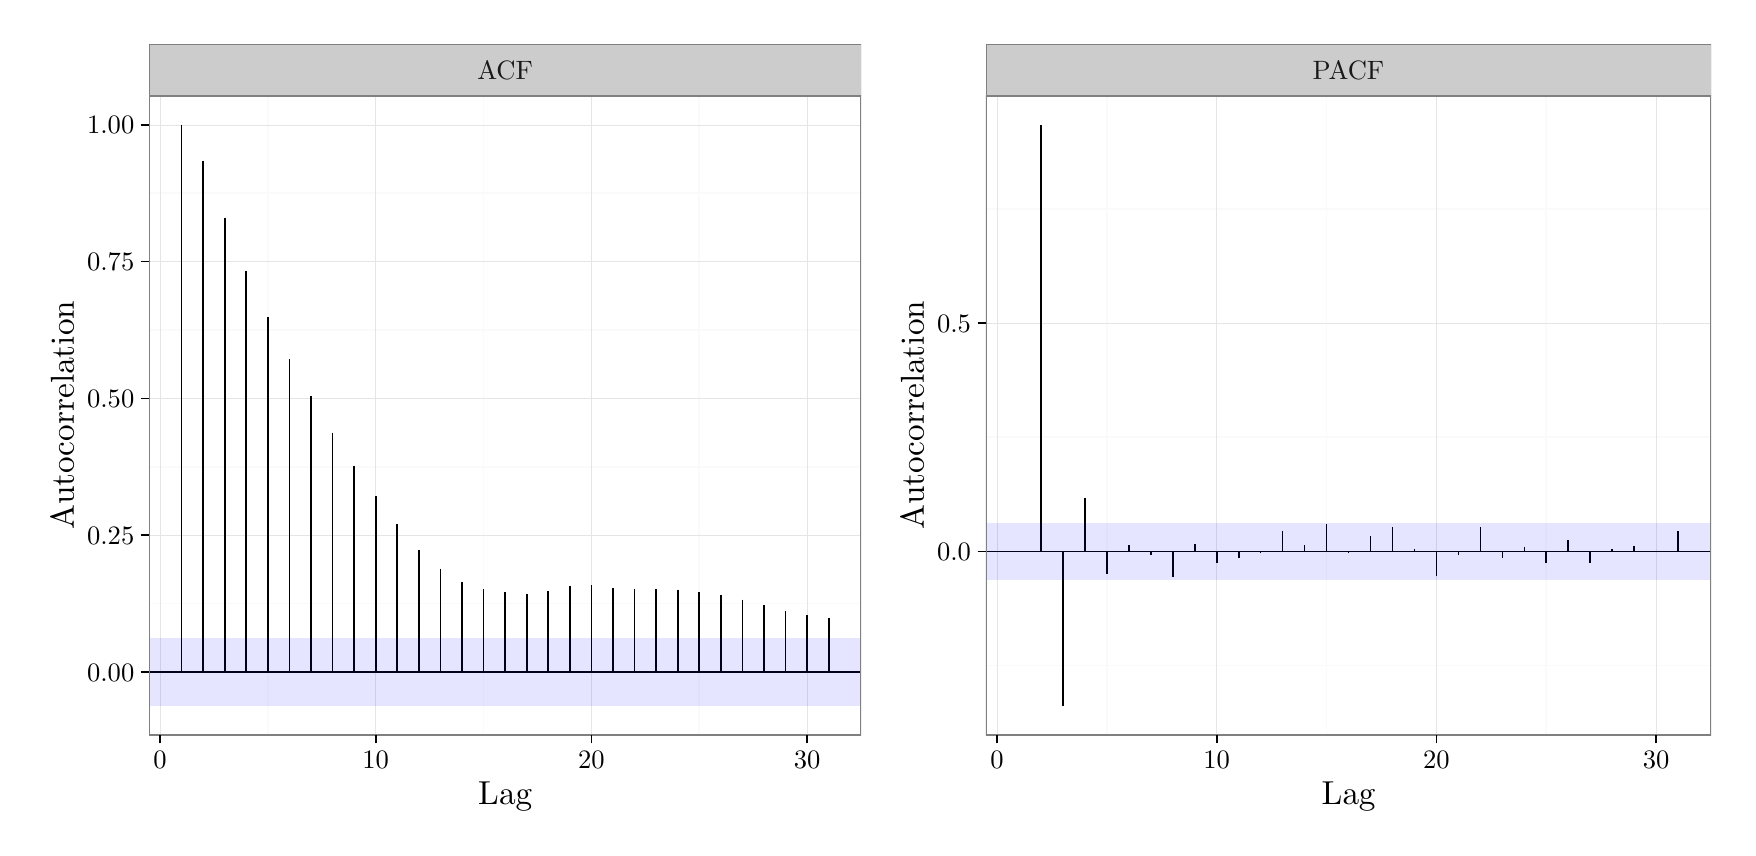
\begin{tikzpicture}[x=1pt,y=1pt]
\definecolor{fillColor}{RGB}{255,255,255}
\path[use as bounding box,fill=fillColor,fill opacity=0.00] (0,0) rectangle (614.29,289.08);
\begin{scope}
\path[clip] (  0.00,  0.00) rectangle (307.15,289.08);
\definecolor{drawColor}{RGB}{255,255,255}
\definecolor{fillColor}{RGB}{255,255,255}

\path[draw=drawColor,line width= 0.6pt,line join=round,line cap=round,fill=fillColor] ( -0.00,  0.00) rectangle (307.15,289.08);
\end{scope}
\begin{scope}
\path[clip] ( 43.93, 33.48) rectangle (301.15,264.47);
\definecolor{fillColor}{RGB}{255,255,255}

\path[fill=fillColor] ( 43.93, 33.48) rectangle (301.15,264.47);
\definecolor{drawColor}{gray}{0.98}

\path[draw=drawColor,line width= 0.6pt,line join=round] ( 43.93, 80.95) --
	(301.15, 80.95);

\path[draw=drawColor,line width= 0.6pt,line join=round] ( 43.93,130.38) --
	(301.15,130.38);

\path[draw=drawColor,line width= 0.6pt,line join=round] ( 43.93,179.82) --
	(301.15,179.82);

\path[draw=drawColor,line width= 0.6pt,line join=round] ( 43.93,229.25) --
	(301.15,229.25);

\path[draw=drawColor,line width= 0.6pt,line join=round] ( 86.80, 33.48) --
	( 86.80,264.47);

\path[draw=drawColor,line width= 0.6pt,line join=round] (164.74, 33.48) --
	(164.74,264.47);

\path[draw=drawColor,line width= 0.6pt,line join=round] (242.69, 33.48) --
	(242.69,264.47);
\definecolor{drawColor}{gray}{0.90}

\path[draw=drawColor,line width= 0.2pt,line join=round] ( 43.93, 56.23) --
	(301.15, 56.23);

\path[draw=drawColor,line width= 0.2pt,line join=round] ( 43.93,105.67) --
	(301.15,105.67);

\path[draw=drawColor,line width= 0.2pt,line join=round] ( 43.93,155.10) --
	(301.15,155.10);

\path[draw=drawColor,line width= 0.2pt,line join=round] ( 43.93,204.53) --
	(301.15,204.53);

\path[draw=drawColor,line width= 0.2pt,line join=round] ( 43.93,253.97) --
	(301.15,253.97);

\path[draw=drawColor,line width= 0.2pt,line join=round] ( 47.82, 33.48) --
	( 47.82,264.47);

\path[draw=drawColor,line width= 0.2pt,line join=round] (125.77, 33.48) --
	(125.77,264.47);

\path[draw=drawColor,line width= 0.2pt,line join=round] (203.72, 33.48) --
	(203.72,264.47);

\path[draw=drawColor,line width= 0.2pt,line join=round] (281.66, 33.48) --
	(281.66,264.47);
\definecolor{drawColor}{RGB}{0,0,0}

\path[draw=drawColor,line width= 0.6pt,line join=round] ( 43.93, 56.23) -- (301.15, 56.23);

\path[draw=drawColor,line width= 0.6pt,line join=round] ( 55.62,253.97) -- ( 55.62, 56.23);

\path[draw=drawColor,line width= 0.6pt,line join=round] ( 63.41,240.90) -- ( 63.41, 56.23);

\path[draw=drawColor,line width= 0.6pt,line join=round] ( 71.21,220.14) -- ( 71.21, 56.23);

\path[draw=drawColor,line width= 0.6pt,line join=round] ( 79.00,201.27) -- ( 79.00, 56.23);

\path[draw=drawColor,line width= 0.6pt,line join=round] ( 86.80,184.38) -- ( 86.80, 56.23);

\path[draw=drawColor,line width= 0.6pt,line join=round] ( 94.59,169.32) -- ( 94.59, 56.23);

\path[draw=drawColor,line width= 0.6pt,line join=round] (102.39,155.92) -- (102.39, 56.23);

\path[draw=drawColor,line width= 0.6pt,line join=round] (110.18,142.79) -- (110.18, 56.23);

\path[draw=drawColor,line width= 0.6pt,line join=round] (117.98,130.68) -- (117.98, 56.23);

\path[draw=drawColor,line width= 0.6pt,line join=round] (125.77,119.72) -- (125.77, 56.23);

\path[draw=drawColor,line width= 0.6pt,line join=round] (133.56,109.60) -- (133.56, 56.23);

\path[draw=drawColor,line width= 0.6pt,line join=round] (141.36,100.50) -- (141.36, 56.23);

\path[draw=drawColor,line width= 0.6pt,line join=round] (149.15, 93.65) -- (149.15, 56.23);

\path[draw=drawColor,line width= 0.6pt,line join=round] (156.95, 88.81) -- (156.95, 56.23);

\path[draw=drawColor,line width= 0.6pt,line join=round] (164.74, 86.33) -- (164.74, 56.23);

\path[draw=drawColor,line width= 0.6pt,line join=round] (172.54, 85.05) -- (172.54, 56.23);

\path[draw=drawColor,line width= 0.6pt,line join=round] (180.33, 84.60) -- (180.33, 56.23);

\path[draw=drawColor,line width= 0.6pt,line join=round] (188.13, 85.62) -- (188.13, 56.23);

\path[draw=drawColor,line width= 0.6pt,line join=round] (195.92, 87.39) -- (195.92, 56.23);

\path[draw=drawColor,line width= 0.6pt,line join=round] (203.72, 87.63) -- (203.72, 56.23);

\path[draw=drawColor,line width= 0.6pt,line join=round] (211.51, 86.50) -- (211.51, 56.23);

\path[draw=drawColor,line width= 0.6pt,line join=round] (219.30, 86.11) -- (219.30, 56.23);

\path[draw=drawColor,line width= 0.6pt,line join=round] (227.10, 86.08) -- (227.10, 56.23);

\path[draw=drawColor,line width= 0.6pt,line join=round] (234.89, 85.98) -- (234.89, 56.23);

\path[draw=drawColor,line width= 0.6pt,line join=round] (242.69, 85.19) -- (242.69, 56.23);

\path[draw=drawColor,line width= 0.6pt,line join=round] (250.48, 84.11) -- (250.48, 56.23);

\path[draw=drawColor,line width= 0.6pt,line join=round] (258.28, 82.40) -- (258.28, 56.23);

\path[draw=drawColor,line width= 0.6pt,line join=round] (266.07, 80.36) -- (266.07, 56.23);

\path[draw=drawColor,line width= 0.6pt,line join=round] (273.87, 78.46) -- (273.87, 56.23);

\path[draw=drawColor,line width= 0.6pt,line join=round] (281.66, 76.70) -- (281.66, 56.23);

\path[draw=drawColor,line width= 0.6pt,line join=round] (289.46, 75.88) -- (289.46, 56.23);
\definecolor{fillColor}{RGB}{0,0,255}

\path[fill=fillColor,fill opacity=0.10] ( 43.93, 43.98) rectangle (301.15, 68.49);
\definecolor{drawColor}{gray}{0.50}

\path[draw=drawColor,line width= 0.6pt,line join=round,line cap=round] ( 43.93, 33.48) rectangle (301.15,264.47);
\end{scope}
\begin{scope}
\path[clip] ( 43.93,264.47) rectangle (301.15,283.08);
\definecolor{drawColor}{gray}{0.50}
\definecolor{fillColor}{gray}{0.80}

\path[draw=drawColor,line width= 0.2pt,line join=round,line cap=round,fill=fillColor] ( 43.93,264.47) rectangle (301.15,283.08);
\definecolor{drawColor}{gray}{0.10}

\node[text=drawColor,anchor=base,inner sep=0pt, outer sep=0pt, scale=  0.96] at (172.54,270.47) {ACF};
\end{scope}
\begin{scope}
\path[clip] (  0.00,  0.00) rectangle (614.29,289.08);
\definecolor{drawColor}{RGB}{0,0,0}

\node[text=drawColor,anchor=base east,inner sep=0pt, outer sep=0pt, scale=  0.96] at ( 38.53, 52.93) {0.00};

\node[text=drawColor,anchor=base east,inner sep=0pt, outer sep=0pt, scale=  0.96] at ( 38.53,102.36) {0.25};

\node[text=drawColor,anchor=base east,inner sep=0pt, outer sep=0pt, scale=  0.96] at ( 38.53,151.79) {0.50};

\node[text=drawColor,anchor=base east,inner sep=0pt, outer sep=0pt, scale=  0.96] at ( 38.53,201.23) {0.75};

\node[text=drawColor,anchor=base east,inner sep=0pt, outer sep=0pt, scale=  0.96] at ( 38.53,250.66) {1.00};
\end{scope}
\begin{scope}
\path[clip] (  0.00,  0.00) rectangle (614.29,289.08);
\definecolor{drawColor}{RGB}{0,0,0}

\path[draw=drawColor,line width= 0.6pt,line join=round] ( 40.93, 56.23) --
	( 43.93, 56.23);

\path[draw=drawColor,line width= 0.6pt,line join=round] ( 40.93,105.67) --
	( 43.93,105.67);

\path[draw=drawColor,line width= 0.6pt,line join=round] ( 40.93,155.10) --
	( 43.93,155.10);

\path[draw=drawColor,line width= 0.6pt,line join=round] ( 40.93,204.53) --
	( 43.93,204.53);

\path[draw=drawColor,line width= 0.6pt,line join=round] ( 40.93,253.97) --
	( 43.93,253.97);
\end{scope}
\begin{scope}
\path[clip] (  0.00,  0.00) rectangle (614.29,289.08);
\definecolor{drawColor}{RGB}{0,0,0}

\path[draw=drawColor,line width= 0.6pt,line join=round] ( 47.82, 30.48) --
	( 47.82, 33.48);

\path[draw=drawColor,line width= 0.6pt,line join=round] (125.77, 30.48) --
	(125.77, 33.48);

\path[draw=drawColor,line width= 0.6pt,line join=round] (203.72, 30.48) --
	(203.72, 33.48);

\path[draw=drawColor,line width= 0.6pt,line join=round] (281.66, 30.48) --
	(281.66, 33.48);
\end{scope}
\begin{scope}
\path[clip] (  0.00,  0.00) rectangle (614.29,289.08);
\definecolor{drawColor}{RGB}{0,0,0}

\node[text=drawColor,anchor=base,inner sep=0pt, outer sep=0pt, scale=  0.96] at ( 47.82, 21.46) {0};

\node[text=drawColor,anchor=base,inner sep=0pt, outer sep=0pt, scale=  0.96] at (125.77, 21.46) {10};

\node[text=drawColor,anchor=base,inner sep=0pt, outer sep=0pt, scale=  0.96] at (203.72, 21.46) {20};

\node[text=drawColor,anchor=base,inner sep=0pt, outer sep=0pt, scale=  0.96] at (281.66, 21.46) {30};
\end{scope}
\begin{scope}
\path[clip] (  0.00,  0.00) rectangle (614.29,289.08);
\definecolor{drawColor}{RGB}{0,0,0}

\node[text=drawColor,anchor=base,inner sep=0pt, outer sep=0pt, scale=  1.20] at (172.54,  8.40) {Lag};
\end{scope}
\begin{scope}
\path[clip] (  0.00,  0.00) rectangle (614.29,289.08);
\definecolor{drawColor}{RGB}{0,0,0}

\node[text=drawColor,rotate= 90.00,anchor=base,inner sep=0pt, outer sep=0pt, scale=  1.20] at ( 16.66,148.97) {Autocorrelation};
\end{scope}
\begin{scope}
\path[clip] (307.15,  0.00) rectangle (614.29,289.08);
\definecolor{drawColor}{RGB}{255,255,255}
\definecolor{fillColor}{RGB}{255,255,255}

\path[draw=drawColor,line width= 0.6pt,line join=round,line cap=round,fill=fillColor] (307.15,  0.00) rectangle (614.29,289.08);
\end{scope}
\begin{scope}
\path[clip] (346.28, 33.48) rectangle (608.30,264.47);
\definecolor{fillColor}{RGB}{255,255,255}

\path[fill=fillColor] (346.28, 33.48) rectangle (608.29,264.47);
\definecolor{drawColor}{gray}{0.98}

\path[draw=drawColor,line width= 0.6pt,line join=round] (346.28, 58.54) --
	(608.30, 58.54);

\path[draw=drawColor,line width= 0.6pt,line join=round] (346.28,141.08) --
	(608.30,141.08);

\path[draw=drawColor,line width= 0.6pt,line join=round] (346.28,223.61) --
	(608.30,223.61);

\path[draw=drawColor,line width= 0.6pt,line join=round] (389.95, 33.48) --
	(389.95,264.47);

\path[draw=drawColor,line width= 0.6pt,line join=round] (469.35, 33.48) --
	(469.35,264.47);

\path[draw=drawColor,line width= 0.6pt,line join=round] (548.75, 33.48) --
	(548.75,264.47);
\definecolor{drawColor}{gray}{0.90}

\path[draw=drawColor,line width= 0.2pt,line join=round] (346.28, 99.81) --
	(608.30, 99.81);

\path[draw=drawColor,line width= 0.2pt,line join=round] (346.28,182.34) --
	(608.30,182.34);

\path[draw=drawColor,line width= 0.2pt,line join=round] (350.25, 33.48) --
	(350.25,264.47);

\path[draw=drawColor,line width= 0.2pt,line join=round] (429.65, 33.48) --
	(429.65,264.47);

\path[draw=drawColor,line width= 0.2pt,line join=round] (509.05, 33.48) --
	(509.05,264.47);

\path[draw=drawColor,line width= 0.2pt,line join=round] (588.45, 33.48) --
	(588.45,264.47);
\definecolor{drawColor}{RGB}{0,0,0}

\path[draw=drawColor,line width= 0.6pt,line join=round] (346.28, 99.81) -- (608.30, 99.81);

\path[draw=drawColor,line width= 0.6pt,line join=round] (366.13,253.97) -- (366.13, 99.81);

\path[draw=drawColor,line width= 0.6pt,line join=round] (374.07, 43.98) -- (374.07, 99.81);

\path[draw=drawColor,line width= 0.6pt,line join=round] (382.01,119.30) -- (382.01, 99.81);

\path[draw=drawColor,line width= 0.6pt,line join=round] (389.95, 91.74) -- (389.95, 99.81);

\path[draw=drawColor,line width= 0.6pt,line join=round] (397.89,102.16) -- (397.89, 99.81);

\path[draw=drawColor,line width= 0.6pt,line join=round] (405.83, 98.46) -- (405.83, 99.81);

\path[draw=drawColor,line width= 0.6pt,line join=round] (413.77, 90.68) -- (413.77, 99.81);

\path[draw=drawColor,line width= 0.6pt,line join=round] (421.71,102.51) -- (421.71, 99.81);

\path[draw=drawColor,line width= 0.6pt,line join=round] (429.65, 95.81) -- (429.65, 99.81);

\path[draw=drawColor,line width= 0.6pt,line join=round] (437.59, 97.54) -- (437.59, 99.81);

\path[draw=drawColor,line width= 0.6pt,line join=round] (445.53, 99.09) -- (445.53, 99.81);

\path[draw=drawColor,line width= 0.6pt,line join=round] (453.47,107.30) -- (453.47, 99.81);

\path[draw=drawColor,line width= 0.6pt,line join=round] (461.41,102.02) -- (461.41, 99.81);

\path[draw=drawColor,line width= 0.6pt,line join=round] (469.35,109.70) -- (469.35, 99.81);

\path[draw=drawColor,line width= 0.6pt,line join=round] (477.29, 99.09) -- (477.29, 99.81);

\path[draw=drawColor,line width= 0.6pt,line join=round] (485.23,105.35) -- (485.23, 99.81);

\path[draw=drawColor,line width= 0.6pt,line join=round] (493.17,108.70) -- (493.17, 99.81);

\path[draw=drawColor,line width= 0.6pt,line join=round] (501.11,100.72) -- (501.11, 99.81);

\path[draw=drawColor,line width= 0.6pt,line join=round] (509.05, 91.09) -- (509.05, 99.81);

\path[draw=drawColor,line width= 0.6pt,line join=round] (516.99, 98.39) -- (516.99, 99.81);

\path[draw=drawColor,line width= 0.6pt,line join=round] (524.93,108.54) -- (524.93, 99.81);

\path[draw=drawColor,line width= 0.6pt,line join=round] (532.87, 97.47) -- (532.87, 99.81);

\path[draw=drawColor,line width= 0.6pt,line join=round] (540.81,101.48) -- (540.81, 99.81);

\path[draw=drawColor,line width= 0.6pt,line join=round] (548.75, 95.70) -- (548.75, 99.81);

\path[draw=drawColor,line width= 0.6pt,line join=round] (556.69,103.86) -- (556.69, 99.81);

\path[draw=drawColor,line width= 0.6pt,line join=round] (564.63, 95.65) -- (564.63, 99.81);

\path[draw=drawColor,line width= 0.6pt,line join=round] (572.57,100.52) -- (572.57, 99.81);

\path[draw=drawColor,line width= 0.6pt,line join=round] (580.51,101.80) -- (580.51, 99.81);

\path[draw=drawColor,line width= 0.6pt,line join=round] (588.45,100.13) -- (588.45, 99.81);

\path[draw=drawColor,line width= 0.6pt,line join=round] (596.39,107.13) -- (596.39, 99.81);
\definecolor{fillColor}{RGB}{0,0,255}

\path[fill=fillColor,fill opacity=0.10] (346.28, 89.58) rectangle (608.29,110.04);
\definecolor{drawColor}{gray}{0.50}

\path[draw=drawColor,line width= 0.6pt,line join=round,line cap=round] (346.28, 33.48) rectangle (608.29,264.47);
\end{scope}
\begin{scope}
\path[clip] (346.28,264.47) rectangle (608.30,283.08);
\definecolor{drawColor}{gray}{0.50}
\definecolor{fillColor}{gray}{0.80}

\path[draw=drawColor,line width= 0.2pt,line join=round,line cap=round,fill=fillColor] (346.28,264.47) rectangle (608.29,283.08);
\definecolor{drawColor}{gray}{0.10}

\node[text=drawColor,anchor=base,inner sep=0pt, outer sep=0pt, scale=  0.96] at (477.29,270.47) {PACF};
\end{scope}
\begin{scope}
\path[clip] (  0.00,  0.00) rectangle (614.29,289.08);
\definecolor{drawColor}{RGB}{0,0,0}

\node[text=drawColor,anchor=base east,inner sep=0pt, outer sep=0pt, scale=  0.96] at (340.88, 96.51) {0.0};

\node[text=drawColor,anchor=base east,inner sep=0pt, outer sep=0pt, scale=  0.96] at (340.88,179.04) {0.5};
\end{scope}
\begin{scope}
\path[clip] (  0.00,  0.00) rectangle (614.29,289.08);
\definecolor{drawColor}{RGB}{0,0,0}

\path[draw=drawColor,line width= 0.6pt,line join=round] (343.28, 99.81) --
	(346.28, 99.81);

\path[draw=drawColor,line width= 0.6pt,line join=round] (343.28,182.34) --
	(346.28,182.34);
\end{scope}
\begin{scope}
\path[clip] (  0.00,  0.00) rectangle (614.29,289.08);
\definecolor{drawColor}{RGB}{0,0,0}

\path[draw=drawColor,line width= 0.6pt,line join=round] (350.25, 30.48) --
	(350.25, 33.48);

\path[draw=drawColor,line width= 0.6pt,line join=round] (429.65, 30.48) --
	(429.65, 33.48);

\path[draw=drawColor,line width= 0.6pt,line join=round] (509.05, 30.48) --
	(509.05, 33.48);

\path[draw=drawColor,line width= 0.6pt,line join=round] (588.45, 30.48) --
	(588.45, 33.48);
\end{scope}
\begin{scope}
\path[clip] (  0.00,  0.00) rectangle (614.29,289.08);
\definecolor{drawColor}{RGB}{0,0,0}

\node[text=drawColor,anchor=base,inner sep=0pt, outer sep=0pt, scale=  0.96] at (350.25, 21.46) {0};

\node[text=drawColor,anchor=base,inner sep=0pt, outer sep=0pt, scale=  0.96] at (429.65, 21.46) {10};

\node[text=drawColor,anchor=base,inner sep=0pt, outer sep=0pt, scale=  0.96] at (509.05, 21.46) {20};

\node[text=drawColor,anchor=base,inner sep=0pt, outer sep=0pt, scale=  0.96] at (588.45, 21.46) {30};
\end{scope}
\begin{scope}
\path[clip] (  0.00,  0.00) rectangle (614.29,289.08);
\definecolor{drawColor}{RGB}{0,0,0}

\node[text=drawColor,anchor=base,inner sep=0pt, outer sep=0pt, scale=  1.20] at (477.29,  8.40) {Lag};
\end{scope}
\begin{scope}
\path[clip] (  0.00,  0.00) rectangle (614.29,289.08);
\definecolor{drawColor}{RGB}{0,0,0}

\node[text=drawColor,rotate= 90.00,anchor=base,inner sep=0pt, outer sep=0pt, scale=  1.20] at (323.81,148.97) {Autocorrelation};
\end{scope}
\end{tikzpicture}
